\documentclass[11pt]{article}

\usepackage{acl}
\usepackage{times}
\usepackage{latexsym}
\usepackage[T1]{fontenc}
\usepackage[utf8]{inputenc}
\usepackage{microtype}
\usepackage{inconsolata}
\usepackage{graphicx}
\usepackage{booktabs}
\usepackage{flushend}
\usepackage{amsmath}
\usepackage{url}

\title{Do Function Vectors and Task Vectors Generalize? \\ A Reproducibility Study Across Model Families and Scale}

\author{Serendeep Rudraraju \\
  University of Marburg \\
  \texttt{rudraraj@students.uni-marburg.de}}

\begin{document}
\maketitle

\begin{abstract}
A language model can learn a task from examples in its prompt. Function vectors (FVs) and task vectors (TVs) aim to transfer that behavior to a new prompt by modifying the model's activations. We reproduce both methods on word-pair tasks across GPT-J, Llama-3.1, and Gemma-2. In held-out tests, FVs outperform random controls on GPT-J and Llama-3.1-8B. TVs outperform shuffled-label controls on GPT-J and both base and instruction-tuned Gemma; the Llama-8B comparison is inconclusive. Our FV implementation achieves zero accuracy on both Gemma checkpoints in a two-task follow-up. Sentiment classification shows a further limitation: in-context learning (ICL) achieves 73.5--94.0\% accuracy with arbitrary labels, while TVs achieve only 49.6--52.7\%. Successful transfer on word pairs therefore does not extend to this sentiment dataset. Separating vector construction, layer selection, and testing also shows why gains over zero-shot accuracy can overstate the evidence for transfer. Code and data are available online.\footnote{\url{https://github.com/Serendeep/fv-tv-repro}}
\end{abstract}

\section{Introduction}
\label{sec:intro}

Ten input-output demonstrations can change how a language model answers a query. Can we transfer that behavior without repeating the demonstrations? \citet{todd2024function} extract a \emph{function vector} (FV) from selected attention heads and add it to the residual stream of a new prompt. \citet{hendel2023incontext} instead extract a \emph{task vector} (TV) from one hidden state and use it to replace a state in the new prompt. Both methods improve task accuracy in the original studies.

The original studies cover GPT-J and several other model families, but leave later checkpoints untested. Interpretability results can depend on metric and intervention choices \citep{zhang2024towards} and vary across models \citep{yin2025which}. We therefore reproduce the effects on GPT-J before extending the same implementation to newer checkpoints.

We ask where these effects hold and what they depend on. We first test 16 word-pair tasks, including antonyms, translation, and capitalization. We then evaluate eight shared tasks with separate data for vector construction, layer selection, and testing. Finally, we test whether TVs transfer sentiment classification when the output labels are arbitrary letters.

Our implementation uses NNsight \citep{fiottokaufman2025nnsight}, with native PyTorch hooks for matched base and instruction-tuned Gemma runs. We compare real vectors with controls that shuffle labels or replace the vector. Further controls change the source task and prompt format. TV experiments also extend to Llama-3.1-70B.

We score the first token of each answer. This measures transfer across the tested tasks and checkpoints, rather than reasoning or open-ended generation. Appendix~\ref{sec:deviations} records departures from the original methods and our sampling protocol \citep{pineau2021improving}.

\section{Background and claims}
\label{sec:claims}

\paragraph{Function vectors.} \citet{todd2024function} first average each attention head's output over demonstration prompts. To identify useful heads, they patch these averages into prompts with shuffled labels. A head's score is the resulting increase in probability of the correct answer, called its average indirect effect (AIE). The FV sums selected head outputs after projection into the residual stream.

Todd et al.\ select heads using AIE averaged across tasks and vary the number of heads, $k$, with model size. Our main grid selects ten heads separately for each task. The original study finds that adding an FV at an early-middle layer restores much of the model's ICL accuracy.

\paragraph{Task vectors.} \citet{hendel2023incontext} append a dummy query to a demonstration prompt. They extract the hidden state $\theta$ at its final token in an intermediate layer $L$. Replacing the corresponding state in a zero-shot prompt with $\theta$ recovers most ICL accuracy. Recovery peaks at intermediate layers and falls at late layers.

FVs add selected head outputs; TVs replace a hidden state. These are activation interventions, distinct from weight-space task arithmetic \citep{ilharco2023editing}. \citet{brumley2024comparing} compare FVs with the in-context vectors of \citet{liu2024incontext}, which use a different construction from Hendel et al.'s TVs.

Related work studies attention heads that support ICL \citep{yin2025which}, their connection to task vectors \citep{yang2025unifying}, and ICL circuits in Gemma-2 2B \citep{bakalova2025contextualize}. \citet{tikhonov2026one} examine TV limits on more complex tasks. Table~\ref{tab:claims} lists the claims we test.

\begin{table*}[t]
  \centering
  \small
  \setlength{\tabcolsep}{3pt}
  \begin{tabular}{p{0.10\linewidth}p{0.70\linewidth}p{0.15\linewidth}}
    \toprule
    \textbf{ID} & \textbf{Claim} & \textbf{Source} \\
    \midrule
    C1.1 & Adding an FV to the residual stream of a zero-shot prompt at an early-middle layer restores a substantial fraction of ICL task accuracy & \citet{todd2024function}, \S\S2.3, 3.1 \\
    C2.1 & Replacing one hidden state of a zero-shot prompt with a TV at an intermediate layer recovers most ICL accuracy & \citet{hendel2023incontext}, \S3 \\
    C2.2 & Recovery is layer-structured: peaks at intermediate layers, collapses late & \citet{hendel2023incontext}, \S3.3 \\
    C3.1 (ours) & FV and TV recovery correlate across tasks within a model & new \\
    C3.2 (ours) & Claims C1.1/C2.1 hold, on the same word-pair tasks, on models neither paper tested: Llama-3.1-8B, Llama-3.1-70B, Gemma-2-9b-it & new \\
    \bottomrule
  \end{tabular}
  \caption{Claims tested in this reproduction.}
  \label{tab:claims}
\end{table*}

\section{Methodology}
\label{sec:method}

We use two evaluation designs. The exploratory grid selects and evaluates layers on the same data. The follow-ups separate construction, development, and test inputs: development accuracy selects the layer, and test accuracy measures transfer. We describe the grid below and the follow-ups in \S\S\ref{sec:heldout}--\ref{sec:sentiment}.

\subsection{Models}

GPT-J-6B \citep{wang2021gptj} is our starting point because both original papers evaluated it. We extend the tests to Llama-3.1-8B \citep{grattafiori2024llama} and Gemma-2-9b-it \citep{gemmateam2024gemma2}. Only Gemma IT is instruction-tuned. The matched Gemma follow-up also tests the base checkpoint. At Llama-3.1-70B, we test TVs only; FV head selection took too long for the available compute time (Appendix~\ref{sec:compute}).

\subsection{Tasks}

The 16 tasks cover linguistic transformations, factual knowledge, translation, and algorithmic sequences (Table~\ref{tab:per-task}). We use the task collection of \citet{todd2024function}, with 197--5{,}199 pairs per task. We compare the top-1 prediction with the first token of the space-prefixed reference. Answers of any length remain in the data, so a correct first token may be only part of an answer such as ``Buenos Aires''.

Within each model, both methods use the same tasks and evaluation splits. Evaluation rows are excluded from demonstrations. Deployment availability determines completed coverage (Table~\ref{tab:protocol}).

\begin{table}[t]
  \centering
  \scriptsize
  \setlength{\tabcolsep}{2.5pt}
  \begin{tabular}{lcccc}
    \toprule
     & \textbf{GPT-J} & \textbf{L3.1-8B} & \textbf{Gemma-2} & \textbf{L3.1-70B} \\
    \midrule
    tasks & 14 & 8 & 5 & 16 \\
    seeds & 0--1 & 0--2 & 0--2 & 0--2 \\
    (task, seed) $n$ & 27 & 24 & 12 & 48 \\
    eval items & 15 & 25 & 25 & 25 \\
    sweep stride & 4 & 2 & 2 & 3 \\
    AIE trials & 5 & 10 & 5 & -- \\
    \bottomrule
  \end{tabular}
  \caption{Exploratory-grid protocol and coverage per model.}
  \label{tab:protocol}
\end{table}

\subsection{Interventions}

Prompts present each demonstration as \texttt{Q: \{x\}\textbackslash nA: \{y\}}, with blank lines between examples. They end with the new query followed by \texttt{A:}. We measure zero-shot accuracy, 10-shot ICL accuracy, and intervention accuracy on the same evaluation split.

FV construction averages head activations over 32 fresh demonstration prompts, then selects the ten highest-AIE heads. TV construction uses one demonstration prompt ending in an in-domain dummy query. Table~\ref{tab:protocol} gives the AIE trials and layer-sweep strides.

We report the fraction of the ICL accuracy gain recovered by the intervention:
\[
  \text{recovery} = \frac{\text{acc}_{\text{method}}-\text{acc}_{\text{zero}}}
                            {\text{acc}_{\text{ICL}}-\text{acc}_{\text{zero}}}.
\]
A ratio above 1 means the intervention exceeds its ICL baseline. The exploratory grid reports the best swept layer.

\subsection{Controls and statistics}

FV controls are a norm-matched Gaussian vector and a random-10-head vector. The TV control permutes demonstration labels among the same inputs, sometimes retaining correct pairs. In the exploratory grid, all controls use the real method's best evaluation layer.

A grid cell is one model--method--task--seed combination. Each exploratory seed draws new demonstrations and evaluation rows. We estimate 95\% intervals by resampling tasks 10,000 times and pooling their seeds. Tasks with more completed seeds therefore receive more weight. Every reported grid cell has an ICL-minus-zero-shot accuracy gap of at least 0.2.

For C1.1 and C2.1, a \emph{pass} requires a positive paired method-minus-control interval and Cohen's $d\geq0.8$. A \emph{weak pass} uses the same interval criterion with $0.5\leq d<0.8$. We average the two FV controls before computing paired differences. Appendix~\ref{sec:panel-analyses} defines the grading and effect sizes.

C2.2 tests the layer profile: TV recovery should peak at intermediate layers and fall toward the end of the model.

Selecting the layer on evaluation data favors the real intervention. We assess this bias by selecting on seed 0 and testing on the remaining seeds (CV in Table~\ref{tab:numbers}). Selecting separately on each evaluation seed raises recovery by 0.00--0.14 on the same cells.

Seed splits can overlap, and this check does not reselect control layers. The follow-up therefore uses a separate development set, as in Hendel et al.\ (\S\ref{sec:heldout}).

\section{Results}
\label{sec:results}

\subsection{Exploratory results}

Both methods reproduce positive effects on GPT-J (Tables~\ref{tab:verdicts} and \ref{tab:numbers}; Figure~\ref{fig:effect-summary}). FV injection recovers 0.50 of the ICL gap ($d=2.4$). TV replacement recovers 0.56, against 0.28 for shuffled states ($d=0.78$), meeting our weak-pass criterion.

TVs show positive paired effects across all four checkpoints in the exploratory grid. FVs also pass on Llama-3.1-8B, with recovery of 0.42 ($d=2.0$), but fail on Gemma-2-9b-it (\S\ref{sec:gemma}). Llama FV recovery ranges from 0.86 on singular-plural to 0.02 on person-occupation. The held-out task results in \S\ref{sec:heldout} examine this variation under balanced coverage.

\begin{table}[t]
  \centering
  \scriptsize
  \setlength{\tabcolsep}{2.5pt}
  \begin{tabular}{lcccc}
    \toprule
    \textbf{Claim} & \textbf{GPT-J} & \textbf{L3.1-8B} & \textbf{Gemma-2} & \textbf{L3.1-70B} \\
    \midrule
    C1.1 (FV) & pass & pass & \textbf{fail} & n/a \\
    C2.1 (TV) & weak pass & pass & pass & pass \\
    C2.2 (layers) & pass & pass & pass & pass \\
    C3.1 (corr.) & \multicolumn{4}{c}{not detected (underpowered; \S\ref{sec:beyond})} \\
    C3.2 (gen.) & \multicolumn{4}{c}{TV qualified; FV mixed} \\
    \bottomrule
  \end{tabular}
  \caption{Exploratory verdicts with evaluation-selected layers. Gemma FV refers to our implementation. Held-out comparisons: \S\ref{sec:heldout}.}
  \label{tab:verdicts}
\end{table}

\begin{table}[t]
  \centering
  \small
  \setlength{\tabcolsep}{4pt}
  \begin{tabular}{llcccc}
\toprule \textbf{Model} & \textbf{M.} & \textbf{Recovery [CI]} & \textbf{CV} & \textbf{Ctrl.} & $d$ \\
\midrule
GPT-J & FV & 0.50 [0.33, 0.65] & 0.58 & -0.01 & 2.43 \\
 & TV & 0.56 [0.41, 0.71] & 0.53 & 0.28 & 0.78 \\
L3.1-8B & FV & 0.42 [0.19, 0.66] & 0.37 & 0.00 & 2.03 \\
 & TV & 0.83 [0.75, 0.91] & 0.77 & 0.42 & 1.68 \\
Gemma-2 & FV & 0.01 [0.00, 0.02] & 0.00 & 0.01 & 0.00 \\
 & TV & 0.83 [0.61, 1.05] & 0.62 & 0.39 & 1.44 \\
L3.1-70B & TV & 0.80 [0.68, 0.90] & 0.68 & 0.48 & 1.03 \\
\bottomrule \end{tabular}

  \caption{Exploratory best-layer recovery and matched controls. CV uses held-out seeds and a different cell subset (Appendix~\ref{sec:panel-analyses}).}
  \label{tab:numbers}
\end{table}

\begin{figure}[t]
  \centering
  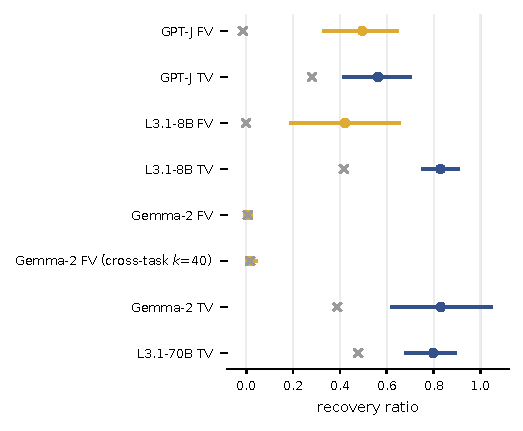
\includegraphics[width=\columnwidth]{figures/effect_summary.pdf}
  \caption{Exploratory best-layer recovery. Bars: task-bootstrap 95\% CIs; $\times$: controls at the same layer; hollow marker: Gemma cross-task heads ($k=40$).}
  \label{fig:effect-summary}
\end{figure}

\subsection{Layer profiles}

\begin{figure}[t]
  \centering
  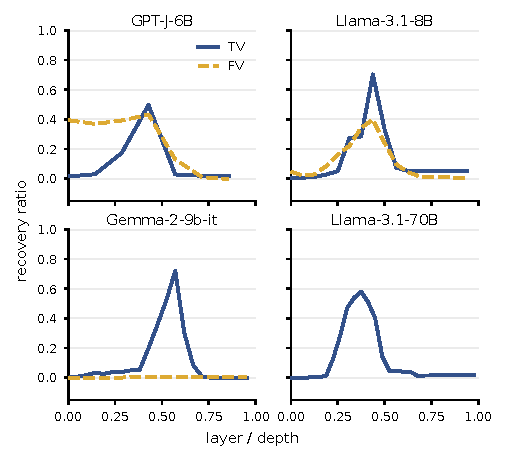
\includegraphics[width=\columnwidth]{figures/layer_profiles.pdf}
  \caption{Exploratory-grid mean recovery by layer depth. FV is dashed; TV is solid.}
  \label{fig:layer-profiles}
\end{figure}

Figure~\ref{fig:layer-profiles} averages recovery at each layer; Table~\ref{tab:numbers} first selects the best layer for each task and seed.

TV recovery peaks at intermediate layers on all four models (Figure~\ref{fig:layer-profiles}): layer 12 of 28 on GPT-J, 14 of 32 on Llama-3.1-8B, 24 of 42 on Gemma-2, and 30 of 80 at 70B. Recovery falls toward the final swept layers, matching C2.2. GPT-J's sweep reaches layer 24.

FV recovery also peaks at intermediate layers on Llama-3.1-8B. GPT-J is flatter, rising from 0.39 at layer 0 to 0.43 at layer 12. Gemma-2 remains near zero throughout.

\begin{figure*}[t]
  \centering
  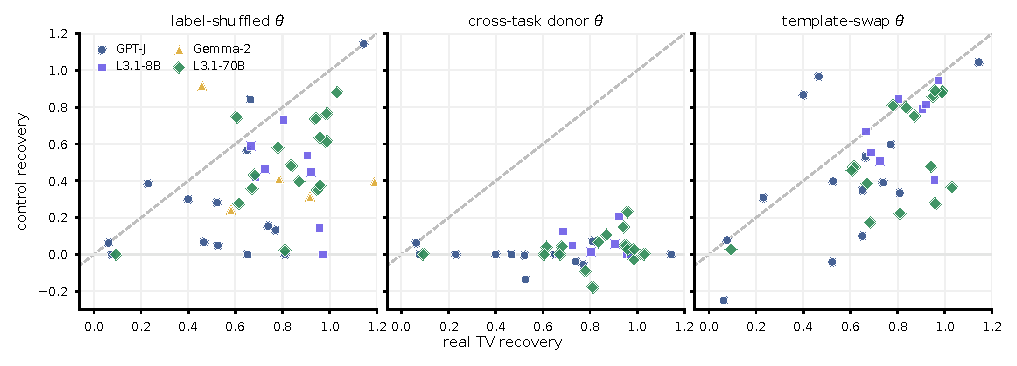
\includegraphics[width=\textwidth]{figures/tv_controls_by_task.pdf}
  \caption{Exploratory TV versus control recovery at the real TV's selected layer. Points average seeds per task and model; the diagonal marks equality.}
  \label{fig:shuffled-theta}
\end{figure*}

\subsection{Function vectors on Gemma-2}
\label{sec:gemma}

Our FV implementation produces little useful transfer on Gemma-2-9b-it. It recovers 0.01 of the ICL gap across 12 cells (95\% CI $[0.00,0.02]$), with zero paired advantage over controls. Scaling the vector, moving the injection site, and selecting up to 40 heads across tasks do not restore a consistent advantage (Appendix~\ref{sec:gemma-diag}).

The matched follow-up tests antonym and country-capital on both Gemma checkpoints, with three seeds and separate development/test inputs. FV accuracy is 0\% throughout, although ICL reaches 68.0--98.7\% (Table~\ref{tab:gemma-fv}). This result applies to our implementation on these two tasks.

\subsection{Additional controls}
\label{sec:beyond}

\paragraph{Recovery after label shuffling.} Shuffled-label states retain 0.28--0.48 recovery across the four models, compared with 0.56--0.83 for correctly labeled states. Shuffling therefore preserves a substantial part of the intervention effect.

The effect varies by task (Figure~\ref{fig:shuffled-theta}; Table~\ref{tab:per-task}). On GPT-J synonym, shuffling reduces recovery from 0.81 to zero. On 70B country-capital, recovery remains 0.88, against 1.03 for the real vector. Task recognition and pretrained associations are possible contributors \citep{pan2023what,min2022rethinking}. In ordinary ICL, label sensitivity also depends on the model and evaluation setup \citep{yoo2022groundtruth,wei2023larger,kossen2024incontext}.

\paragraph{Sibling tasks and extraction templates.} We extract a state from a sibling task, such as synonym for antonym, and patch it at the target task's best layer. Mean recovery is $-0.01$ on GPT-J, 0.06 on Llama-3.1-8B, and 0.03 at 70B (Table~\ref{tab:tv-controls}). Transfer is small on average, with exceptions: present-past vectors recover 0.23 on 70B singular-plural.

A template-swap control extracts from correctly labeled \texttt{x -> y} demonstrations and patches into the usual Q:/A: prompt. Mean recovery is 0.41 on GPT-J, 0.69 on Llama-3.1-8B, and 0.55 at 70B. Both controls use the real vector's selected layer. Appendix~\ref{sec:panel-analyses} specifies donors and prompts.

\begin{table}[t]
  \centering
  \small
  \setlength{\tabcolsep}{4pt}
  \begin{tabular}{lccc}
\toprule \textbf{$\theta$ variant} & \textbf{GPT-J} & \textbf{L3.1-8B} & \textbf{L3.1-70B} \\
\midrule
real, replace & 0.56 & 0.83 & 0.80 \\
label-shuffled & 0.28 & 0.42 & 0.48 \\
cross-task donor & -0.01 & 0.06 & 0.03 \\
template swap & 0.41 & 0.69 & 0.55 \\
real, additive & 0.16 & 0.42 & 0.49 \\
\midrule cells / tasks & 27 / 14 & 24 / 8 & 48 / 16 \\
\bottomrule \end{tabular}

  \caption{Exploratory control recovery at the real TV's best layer; additive TV selects its own best layer. Means across cells.}
  \label{tab:tv-controls}
\end{table}

\paragraph{Surface edits depend on extraction format.} On GPT-J, changing Q:/A: extraction to the arrow template raises capitalization recovery from 0.47 to 0.97 and first-letter capitalization from 0.40 to 0.87. These apparent failures depend on the extraction format. Lowercasing the first letter remains weak under both templates: recovery is 0.23 and 0.31 on GPT-J, and 0.09 and 0.03 at 70B.

Adding the TV instead of replacing the state improves only one of six surface-edit task-model averages: full capitalization at 70B, from 0.78 to 0.82. Appendix~\ref{sec:panel-analyses} gives all additive results.

\paragraph{Cross-method correlation (C3.1).} Per-task FV and TV recovery have Spearman $\rho=0.05$ on GPT-J ($p=0.86$, 14 tasks) and $\rho=-0.05$ on Llama-3.1-8B ($p=0.91$, eight tasks). These small samples provide no evidence of correlation and have limited power to detect one.

\subsection{Held-out evaluation}
\label{sec:heldout}

Does the advantage over controls survive independent layer selection? We construct vectors on one input set, select layers on development inputs, and evaluate once on test inputs. Each control selects its own layer. The sets are disjoint.

We complete 96 cells across two models, two methods, eight tasks, and three construction seeds. Each task reserves 25 development inputs and 50 test inputs. Appendix~\ref{sec:heldout-protocol} gives the partitions and construction details.

\begin{table}[t]
  \centering
  \small
  \setlength{\tabcolsep}{4pt}
  \begin{tabular}{llrr}
\toprule
Model & Method & Difference & 95\% CI \\
\midrule
GPT-J & FV & $+35.9$ & $[18.5, 52.6]$ \\
GPT-J & TV & $+16.1$ & $[4.1, 30.3]$ \\
Llama-3.1-8B & FV & $+24.3$ & $[7.6, 42.9]$ \\
Llama-3.1-8B & TV & $-4.2$ & $[-20.7, 8.7]$ \\
\bottomrule
\end{tabular}

  \caption{Held-out method-minus-control accuracy (percentage points). Each control selects its own layer; 95\% CIs bootstrap eight task means.}
  \label{tab:heldout}
\end{table}

FVs exceed the mean of their random controls on both models (Table~\ref{tab:heldout}). TVs exceed shuffled-label controls on GPT-J, while the Llama interval crosses zero.

The Llama result shows why control layers matter. TV accuracy is 50.0\%; shuffled controls reach 54.2\% at their own selected layers, but only 34.7\% at the real TV's selected layer. TV accuracy remains well above the 4.1\% zero-shot baseline without an established advantage over shuffling.

Task differences remain large (Table~\ref{tab:heldout-tasks}). On Llama, the TV-minus-shuffle difference is $-55.6$ points for English-French and $+21.8$ for antonym. The aggregate result therefore does not describe a uniform failure across tasks.

\subsection{Matched Gemma task-vector evaluation}
\label{sec:gemma-heldout}

Both Gemma checkpoints follow the same eight-task protocol, giving 48 TV cells. They share input partitions and demonstrations, and each control selects its own layer. Both run in FP16 on the same hardware and software setup. We specified this extension after inspecting the earlier follow-up; Appendix~\ref{sec:extension-protocol} records the backend checks.

\begin{table}[t]
  \centering
  \scriptsize
  \setlength{\tabcolsep}{3pt}
  \begin{tabular}{lrrrr}
\toprule
Model & TV & Control & $\Delta$ & 95\% CI \\
\midrule
Gemma base & 62.6 & 43.6 & $+19.1$ & $[3.9,35.3]$ \\
Gemma IT & 66.4 & 34.0 & $+32.3$ & $[7.4,57.9]$ \\
\bottomrule
\end{tabular}

  \caption{Held-out Gemma TV accuracy (\%). $\Delta$: TV minus independently selected shuffled controls (percentage points); 95\% CIs bootstrap tasks.}
  \label{tab:gemma-heldout}
\end{table}

TVs exceed shuffled controls by 19.1 points on base Gemma and 32.3 on Gemma IT (Table~\ref{tab:gemma-heldout}). The larger IT advantage is uncertain: the paired difference is 13.3 points, with a task-bootstrap interval of $[-2.9,27.9]$. Per-task results appear in Table~\ref{tab:gemma-tasks}.

\subsection{Sentiment and arbitrary label mappings}
\label{sec:sentiment}

Word pairs often have familiar answers. Sentiment classification lets us test transfer with unfamiliar output labels. We use short movie-review texts from the SST-2-derived dataset released by \citet{todd2024function}. In one condition, positive reviews map to A and negative reviews to B. A second condition reverses the mapping. We also test the natural labels, positive and negative. Arbitrary labels probe reliance on familiar label meanings in ICL \citep{wei2023larger}.

All conditions use the same inputs and construction choices. Each model receives ten balanced demonstrations, with 40 balanced development inputs and 80 balanced test inputs. Four checkpoints, three label mappings, and three construction seeds give 36 cells. Appendix~\ref{sec:extension-protocol} gives the full protocol.

\begin{figure}[t]
  \centering
  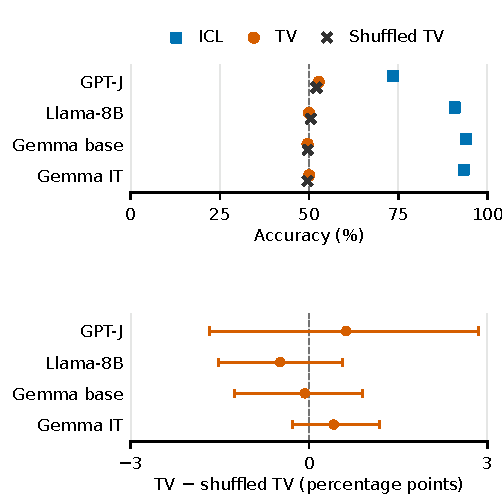
\includegraphics[width=\columnwidth]{figures/sentiment_transfer.pdf}
  \caption{Sentiment with arbitrary labels. Top: accuracy and the 50\% constant-class baseline. Bottom: TV minus shuffled controls, with paired input-bootstrap 95\% CIs. Means combine seeds and mappings.}
  \label{fig:sentiment}
\end{figure}

ICL reaches 73.5--94.0\% with arbitrary labels. TV accuracy stays at 49.6--52.7\%, close to the 50\% constant-class baseline (Figure~\ref{fig:sentiment}). In 18 of 24 arbitrary-label TV cells, the model predicts the same token for every test input. All four intervals for TV minus shuffled controls cross zero. Table~\ref{tab:sentiment-full} gives the per-mapping results.

Natural labels do not rescue transfer: TV accuracy is 50.0\% on GPT-J, Llama-8B, and base Gemma, and 49.2\% on Gemma IT. The failure therefore extends to both natural and arbitrary labels on this dataset, despite strong ICL. These comparisons do not establish statistical equivalence to controls.

\section{Discussion}
\label{sec:discussion}

Gains over zero-shot accuracy alone can overstate transfer. On Llama-8B, TVs improve accuracy without an established advantage over shuffled demonstrations. Both Gemma checkpoints retain an advantage on word pairs, but all four checkpoints transfer little sentiment behavior. Giving each control its own development-selected layer makes these comparisons less dependent on the real vector's preferred site.

The observed limits differ across tasks. Changing the extraction template restores recovery on two weak capitalization tasks, while sentiment transfer remains weak with both natural and arbitrary labels. Label shuffling preserves part of the effect on many word-pair tasks. These patterns support testing transfer across demonstration content and format, consistent with broader studies of steering reliability \citep{tan2024analysing}. FV and TV effect sizes remain distinct because their controls differ.

\section{Conclusion}
\label{sec:conclusion}

FV and TV transfer holds on several word-pair tasks, with different limits across checkpoints. FVs beat random controls on GPT-J and Llama-8B, but our Gemma implementation fails in the two-task follow-up. TVs beat shuffled controls on GPT-J and both Gemma checkpoints; the Llama-8B comparison is inconclusive. On sentiment, all four checkpoints show strong ICL but weak TV transfer. A successful intervention on word pairs is therefore insufficient evidence of broader task transfer.

\section*{Acknowledgments}

We thank the NDIF and NNsight teams for model access, shared no-cost compute, and technical support. LLMs assisted with framing the study, developing code, and cross-checking the analysis.

\section*{Limitations}

\paragraph{Scope.} The study covers word-pair tasks and one SST-2-derived sentiment dataset, scored by first-token accuracy. It does not evaluate complete multi-token answers, reasoning, or open-ended generation. Coverage remains unequal: the matched Gemma FV extension has only two tasks, while Gemma TV covers eight. The extensions were selected after earlier results were available and are reported separately.

\paragraph{FV implementation.} Our implementation selects ten heads per task and does not filter prompts by ICL correctness. Both choices differ from Todd et al.'s main recipe. The Gemma cross-task check also retains prompt differences and uses five AIE trials. The Gemma result does not identify the cause of failure, including possible effects of normalization and head selection (Appendix~\ref{sec:deviations}).

\paragraph{Controls.} Shuffling preserves the input and output sets and can retain correct pairings. Sibling-task donors also change vocabulary and prompts, while template swaps use correct labels. These controls cannot isolate task-rule information from task recognition or pretrained associations. We use one shuffle per exploratory cell and three per held-out cell.

\paragraph{Evaluation.} The exploratory grid selects layers on evaluation data, which can also overlap FV AIE queries. Held-out evaluation removes that overlap but changes sampling, AIE trials, and layer sweeps. Differences between the two evaluations cannot be attributed to splitting alone. The task datasets had also been explored before the follow-up.

\paragraph{Uncertainty.} Construction seeds reuse test inputs, so they do not provide independent test samples. Exploratory task-bootstrap intervals use 5--16 task clusters; held-out intervals use eight. Sentiment intervals measure uncertainty across inputs, with seeds and label mappings held fixed. Two FV tasks are too few to estimate uncertainty across tasks. The FP16 native-hook and NDIF backends also have numerical differences (Appendix~\ref{sec:extension-protocol}).

\bibliography{references}

\appendix

\section{Method and protocol differences}
\label{sec:deviations}

We distinguish departures from the original FV/TV methods from changes to our intended sampling protocol.

\paragraph{Sampling.} The intended grid used 25 evaluation items, seeds 0--2, stride-2 layer sweeps, and ten AIE trials. GPT-J used 15 items, two seeds, stride 4, and five AIE trials. Gemma used five AIE trials and completed 12 of 15 cells. The 70B sweep used stride 3. Deployment availability limited coverage.

\paragraph{FV construction.} The main grid selects ten heads separately for each task. The Gemma cross-task check instead averages AIE over five tasks and uses $k=10,20,40$. Exploratory AIE queries can overlap evaluation inputs.

Todd et al.\ filter for successful ICL in their stated construction (\S2.2) and headline evaluation (\S3.1), with an unfiltered evaluation in Appendix D. We do not apply this filter. We also fix demonstrations within each evaluation split, while their FV pipeline resamples them per query. Our mean-activation and AIE steps do resample prompts.

\paragraph{TV construction.} We use Q:/A: prompts and Todd et al.'s task collection. Hendel et al.\ use an arrow separator and a different task suite. They restrict outputs to single tokens, while we retain answers of any length and score the first token. Our exploratory control uses one ordinary label permutation at the real TV's selected layer. Neither study's authors were contacted.

\paragraph{Intervention mechanics.} We exclude the output-projection bias from per-head contributions to avoid counting it $k$ times when summing $k$ heads. Head dimensions come from the model configuration: $d_{\text{model}}/n_{\text{heads}}$ gives the wrong width for Gemma-2. TV extraction ends with an in-domain dummy query excluded from its demonstrations.

\paragraph{Batching.} We batch per-head AIE patches and reduce the batch size after memory errors. For 70B, cross-layer tensors move to a common device before stacking. These adjustments preserve the intervention definition.

\section{Compute}
\label{sec:compute}

The exploratory grid and initial held-out evaluation use NDIF's shared model deployments. Each traced forward pass is one remote job. A job took roughly 18 seconds, including queueing and download.

FV head search dominates the cost. On Gemma-2, one task and seed under the full protocol requires about 1,400 jobs. This cost motivated the smaller evaluation sets, strided sweeps, and TV-only scope at 70B. The exploratory grid used roughly 21,000 jobs over three days. This estimate excludes the held-out evaluation.

The GPT-J held-out FV runs required smaller AIE batches after memory errors. The matched Gemma extensions use two Kaggle T4 GPUs, with layers split across devices. They use no quantization or CPU/disk offloading.

\section{Gemma-2 diagnostics}
\label{sec:gemma-diag}

We first test whether the FV write changes model predictions, then vary its magnitude, injection site, and head selection. The initial antonym checks use seed 0 and 15 evaluation items. Prediction flips are diagnostic counts, not significance tests.

\paragraph{Positive control.} A random vector scaled to the residual norm changes 3--6 of 15 predictions per layer. This vector is 10--46 times larger than the FV. The result confirms that the write path can affect predictions at that scale.

\paragraph{Vector magnitude.} The FV norm is 10.4, compared with residual norms of 107--474. Multiplying the FV by $\alpha\in\{1,2,4,8\}$ leaves recovery at zero at every tested layer. The larger multipliers bring it near the residual norm at early layers.

\paragraph{Injection site.} Gemma-2 applies RMSNorm after the attention output projection and before the residual addition. Adding projected head outputs directly to the residual stream skips this normalization.

Injecting before RMSNorm changes 1--4 predictions but still gives zero recovery. At the deepest probe layer, it changes 4 of 15 predictions, compared with 6 for the random control.

\paragraph{Country-capital check.} The second task shows the same norm and injection-site pattern. We did not run its strength sweep. Its residual-scale random control changes only 0--3 of 15 predictions, so the clearest write-path evidence comes from antonym.

\paragraph{Shared head selection.} The cross-task check uses antonym, capitalize, country-capital, next-item, and synonym. Each uses seed 0, 25 evaluation items, 32 mean-activation prompts, five AIE trials, and 16-row AIE batches.

We average the five AIE maps and select the top $k$ heads for $k=10,20,40$. Each task builds its FV from its own mean activations over that shared head set. We test every second injection layer.

The largest per-task AIE scores are 0.071 for antonym, 0.265 for capitalize, 0.032 for country-capital, 0.033 for next-item, and 0.014 for synonym. The selected heads lie in layers 24--32 at $k=10$ and 17--41 at $k=40$. Vector norms increase from 10 to 28.

Best-layer recovery remains 0.00 except on synonym, where it is 0.08 at all three values of $k$. Random-control recovery is 0.00 except on synonym at $k=40$, where it also reaches 0.08.

\section{Additional analyses}
\label{sec:panel-analyses}

\begin{table*}[t]
  \centering
  \small
  \setlength{\tabcolsep}{4pt}
  \begin{tabular}{lcccccccc}
\toprule
 & \multicolumn{2}{c}{\textbf{GPT-J}} & \multicolumn{2}{c}{\textbf{L3.1-8B}} & \multicolumn{2}{c}{\textbf{Gemma-2}} & \multicolumn{2}{c}{\textbf{L3.1-70B}} \\
\textbf{Task} & TV & shuf. & TV & shuf. & TV & shuf. & TV & shuf. \\
\midrule
\multicolumn{9}{l}{\emph{linguistic}} \\
antonym & 0.77 & 0.13 & 0.91 & 0.54 & 0.79 & 0.41 & 0.95 & 0.35 \\
synonym & 0.81 & 0.00 & 0.73 & 0.47 & 0.58 & 0.24 & 0.84 & 0.48 \\
present-past & 0.08 & 0.00 & 0.97 & 0.00 & -- & -- & 0.99 & 0.61 \\
singular-plural & 0.53 & 0.05 & 0.69 & 0.42 & -- & -- & 0.96 & 0.64 \\
\multicolumn{9}{l}{\emph{knowledge}} \\
country-capital & 0.74 & 0.15 & 0.96 & 0.14 & 0.92 & 0.31 & 1.03 & 0.88 \\
country-currency & 0.06 & 0.06 & -- & -- & -- & -- & 0.81 & 0.02 \\
person-occupation & 1.14 & 1.14 & 0.67 & 0.59 & -- & -- & 0.61 & 0.75 \\
park-country & -- & -- & -- & -- & -- & -- & 0.99 & 0.77 \\
\multicolumn{9}{l}{\emph{translation}} \\
english-french & 0.66 & 0.84 & 0.80 & 0.73 & -- & -- & 0.96 & 0.38 \\
english-spanish & -- & -- & -- & -- & -- & -- & 0.94 & 0.74 \\
english-german & 0.65 & 0.57 & -- & -- & -- & -- & 0.68 & 0.43 \\
\multicolumn{9}{l}{\emph{algorithmic}} \\
capitalize & 0.47 & 0.07 & -- & -- & 0.46$^{\dagger}$ & 0.92 & 0.78 & 0.58 \\
capitalize-first-letter & 0.40 & 0.30 & -- & -- & -- & -- & 0.61 & 0.28 \\
lowercase-first-letter & 0.23$^{\dagger}$ & 0.38 & -- & -- & -- & -- & 0.09 & 0.00 \\
next-item & 0.52 & 0.28 & 0.92 & 0.45 & 1.19 & 0.39 & 0.87 & 0.40 \\
prev-item & 0.65 & 0.00 & -- & -- & -- & -- & 0.67 & 0.36 \\
\bottomrule
\end{tabular}

  \caption{Exploratory TV and shuffled-state recovery at the TV's best layer, averaged over seeds. $^{\dagger}$: one seed; dash: untested.}
  \label{tab:per-task}
\end{table*}

\paragraph{Paired differences.} Table~\ref{tab:paired-grid} reports the task-bootstrap comparisons used for exploratory grading. Every Gemma FV cell has a zero paired difference, so its confidence interval is $[0,0]$.

\begin{table}[t]
  \centering
  \small
  \input{generated/paired_grid_table}
  \caption{Exploratory method-minus-control recovery and task-bootstrap 95\% CIs.}
  \label{tab:paired-grid}
\end{table}

Cohen's $d$ uses a pooled standard deviation, with both FV controls treated as control observations. It is a descriptive effect size. The paired task-bootstrap interval supplies the uncertainty estimate.

Arms with fewer than five tasks receive \emph{insufficient data}. Otherwise, an arm that meets neither pass threshold receives \emph{fail}. This grade does not establish equivalence to controls.

\paragraph{Sampling and layer selection.} TV extraction reserves 50 rows before sampling demonstrations. ICL reserves only the arm's 15 or 25 evaluation rows. The demonstration sets can therefore differ, although both exclude evaluation rows and remain fixed within a split.

The CV and headline columns in Table~\ref{tab:numbers} cover different cells. Their difference is not an estimate of layer-selection bias.

\paragraph{Small baseline gaps.} Excluding cells with $\text{ICL}-\text{zero}<0.2$ removes no cells from the main results. The recovery estimates and shuffled-state results are unchanged.

\paragraph{Coverage.} Table~\ref{tab:per-task} identifies the tested tasks and missing cells. GPT-J covers 14 tasks and 27 task--seed pairs, Llama-8B covers 8 and 24, and Gemma covers 5 and 12. The 70B TV arm covers all 16 tasks and 48 pairs.

\paragraph{Additional TV controls.} These controls cover every exploratory TV cell on GPT-J, Llama-8B, and Llama-70B. They reuse each cell's ICL baseline, zero-shot baseline, and selected layer.

For cross-task transfer, the donor TV uses its own demonstrations and dummy query at the target seed. Table~\ref{tab:donors} gives the task mapping. We patch the donor state at the target TV's selected layer.

\begin{table}[t]
  \centering
  \small
  \setlength{\tabcolsep}{3pt}
  \begin{tabular}{ll}
    \toprule
    Task & Donor \\
    \midrule
    antonym & synonym \\
    present-past & singular-plural \\
    country-capital & country-currency \\
    person-occupation & park-country \\
    english-french & english-german \\
    capitalize & capitalize-first \\
    next-item & previous-item \\
    \midrule
    english-spanish & english-french \\
    lowercase-first & capitalize-first \\
    \bottomrule
  \end{tabular}
  \caption{Cross-task donors. The first seven pairs also run in reverse.}
  \label{tab:donors}
\end{table}

The template control keeps the real TV's demonstrations and dummy query, but formats them as \texttt{x -> y} lines ending with \texttt{q ->}. The additive variant adds the real TV at the final token instead of replacing the state, and selects its best swept layer.

\begin{table}[t]
  \centering
  \small
  \begin{tabular}{lrrrr}
    \toprule
     & \multicolumn{2}{c}{GPT-J} & \multicolumn{2}{c}{70B} \\
    Task & Add & Replace & Add & Replace \\
    \midrule
    capitalize & 0.07 & 0.47 & 0.82 & 0.78 \\
    capitalize-first & 0.17 & 0.40 & 0.21 & 0.61 \\
    lowercase-first & 0.00 & 0.23 & 0.04 & 0.09 \\
    \bottomrule
  \end{tabular}
  \caption{Best-layer TV recovery on surface edits, averaged over seeds.}
  \label{tab:additive}
\end{table}

Table~\ref{tab:additive} compares additive and replacement recovery on surface edits. Only 70B capitalization improves with addition.

\section{Held-out protocol and task results}
\label{sec:heldout-protocol}

\begin{table*}[t]
  \centering
  \small
  \begin{tabular}{llrrrrr}
\toprule
Model & Method & Zero-shot & ICL & Real & Control (own) & Control (real) \\
\midrule
GPT-J & FV & 6.6 & 72.4 & 43.4 & 7.5 & 7.4 \\
GPT-J & TV & 6.6 & 72.4 & 47.0 & 30.9 & 25.7 \\
Llama-3.1-8B & FV & 4.1 & 83.7 & 28.6 & 4.3 & 3.8 \\
Llama-3.1-8B & TV & 4.1 & 83.7 & 50.0 & 54.2 & 34.7 \\
\bottomrule
\end{tabular}

  \caption{Held-out accuracy (\%), averaged over seeds and tasks. Control (own) uses each control's selected layer; control (real) uses the real method's layer.}
  \label{tab:heldout-accuracy}
\end{table*}

\begin{table*}[t]
  \centering
  \small
  \begin{tabular}{lrrrr}
\toprule
Task & GPT-J FV & GPT-J TV & Llama-3.1-8B FV & Llama-3.1-8B TV \\
\midrule
antonym & $+38.0$ & $+14.4$ & $+38.3$ & $+21.8$ \\
country-capital & $+76.7$ & $+56.4$ & $+4.3$ & $-3.1$ \\
english-french & $+26.0$ & $+3.6$ & $+0.7$ & $-55.6$ \\
next-item & $+45.3$ & $-9.2$ & $+55.3$ & $+9.2$ \\
person-occupation & $+0.0$ & $+3.3$ & $+0.0$ & $-6.4$ \\
present-past & $+43.3$ & $+29.3$ & $+5.7$ & $+8.4$ \\
singular-plural & $+56.7$ & $+23.3$ & $+69.7$ & $-11.3$ \\
synonym & $+1.3$ & $+7.8$ & $+20.3$ & $+3.6$ \\
\bottomrule
\end{tabular}

  \caption{Held-out method-minus-control accuracy (percentage points), averaged over seeds. Controls select their own development layers.}
  \label{tab:heldout-tasks}
\end{table*}

\paragraph{Input partitions.} We fix the tasks, partitions, construction seeds, and analysis before the follow-up. Partition seed 20260905 groups exact input strings and removes duplicate identical pairs. It assigns 50 input groups to test, 25 to development, and the rest to construction.

Alternate outputs stay with the same input. Thus, next-item has 53 test rows and 26 development rows, while the other tasks have 50 and 25. All models and methods use the same partitions. Construction seeds are 100--102.

\paragraph{TV construction.} Each TV and its ICL baseline share ten construction demonstrations. A separate construction input provides the dummy query. Three ordinary permutations shuffle the same labels while keeping inputs and the dummy query fixed. Some correct pairings can remain.

\paragraph{FV construction.} We use 32 mean-activation prompts and ten AIE trials, all drawn from construction inputs. Each task selects its top ten heads without filtering for ICL correctness. Controls use a norm-matched Gaussian vector and a random-ten-head vector. The FV procedure resamples prompts independently of the TV demonstrations.

\paragraph{Layer selection.} We test each intervention and control at every fourth layer and the final layer. Each intervention and control selects its highest-accuracy development layer, with ties resolved toward the lowest layer. We freeze the choices before testing.

As a secondary comparison, we also test controls at the real intervention's selected layer. Test accuracy never selects a layer.

\paragraph{Averaging results.} The primary statistic subtracts mean control accuracy from real-intervention accuracy, using the layer selected separately for each intervention and control. We first average seeds within tasks, then give each task equal weight.

Percentile 95\% intervals use 10,000 bootstrap resamples of the eight task means (seed 20260905). We assign no pass/fail grades because the task count limits interval precision. Secondary recovery ratios require a positive ICL-minus-zero-shot gap, which all 96 cells satisfy.

\section{Matched Gemma and sentiment extension protocols}
\label{sec:extension-protocol}

\begin{table*}[t]
  \centering
  \small
  \begin{tabular}{lrrrrrr}
\toprule
Task & Base ICL & Base TV & Base ctrl. & IT ICL & IT TV & IT ctrl. \\
\midrule
antonym & 70.0 & 60.0 & 42.2 & 68.0 & 42.0 & 55.6 \\
country-capital & 98.7 & 94.0 & 87.8 & 90.7 & 84.7 & 85.1 \\
english-french & 92.7 & 79.3 & 58.9 & 91.3 & 86.7 & 21.6 \\
next-item & 90.6 & 62.3 & 18.0 & 94.3 & 83.0 & 16.1 \\
person-occupation & 63.3 & 25.3 & 40.9 & 60.7 & 23.3 & 28.4 \\
present-past & 98.7 & 72.7 & 14.4 & 99.3 & 90.0 & 9.8 \\
singular-plural & 100.0 & 87.3 & 63.3 & 100.0 & 87.3 & 28.4 \\
synonym & 42.0 & 20.0 & 22.9 & 44.0 & 34.0 & 27.3 \\
\bottomrule
\end{tabular}

  \caption{Gemma TV accuracy (\%), averaged over three seeds. Controls average three shuffled TVs with independently selected layers.}
  \label{tab:gemma-tasks}
\end{table*}

\begin{table*}[t]
  \centering
  \small
  \setlength{\tabcolsep}{4pt}
  \begin{tabular}{llrrrrrrr}
\toprule
Model & Labels & Zero & ICL & TV & Control & $\Delta$ & 95\% CI & Constant \\
\midrule
GPT-J & Natural & 0.0 & 84.6 & 50.0 & 51.4 & $-1.4$ & $[-2.4,-0.6]$ & 3/3 \\
GPT-J & A/B & 0.0 & 86.7 & 57.5 & 55.0 & $+2.5$ & $[-0.6,5.4]$ & 0/3 \\
GPT-J & B/A & 2.5 & 60.4 & 47.9 & 49.2 & $-1.2$ & $[-4.2,1.7]$ & 2/3 \\
Llama-8B & Natural & 0.0 & 93.8 & 50.0 & 51.7 & $-1.7$ & $[-2.9,-0.3]$ & 3/3 \\
Llama-8B & A/B & 0.0 & 91.7 & 50.0 & 51.2 & $-1.2$ & $[-3.3,1.0]$ & 3/3 \\
Llama-8B & B/A & 3.8 & 90.0 & 50.0 & 49.7 & $+0.3$ & $[-1.1,1.7]$ & 3/3 \\
Gemma base & Natural & 0.0 & 93.3 & 50.0 & 55.4 & $-5.4$ & $[-7.8,-2.9]$ & 3/3 \\
Gemma base & A/B & 6.2 & 94.2 & 49.6 & 50.7 & $-1.1$ & $[-2.9,0.6]$ & 2/3 \\
Gemma base & B/A & 7.5 & 93.8 & 49.6 & 48.6 & $+1.0$ & $[-0.6,2.4]$ & 2/3 \\
Gemma IT & Natural & 0.0 & 93.3 & 49.2 & 48.8 & $+0.4$ & $[-0.8,1.4]$ & 1/3 \\
Gemma IT & A/B & 2.5 & 92.9 & 50.0 & 48.9 & $+1.1$ & $[0.4,1.9]$ & 3/3 \\
Gemma IT & B/A & 3.8 & 93.8 & 50.0 & 50.3 & $-0.3$ & $[-1.1,0.7]$ & 3/3 \\
\bottomrule
\end{tabular}

  \caption{Sentiment accuracy (\%), averaged over seeds. $\Delta$: TV minus shuffled controls (percentage points), with stratified input-bootstrap 95\% CIs. Constant: seeds predicting one token throughout.}
  \label{tab:sentiment-full}
\end{table*}

\subsection{Gemma execution checks}

Both Gemma checkpoints use fixed revisions, native PyTorch hooks, FP16 weights, and Q:/A: prompts. Inference uses eager attention, left padding, batches of four, and no KV cache. Both checkpoints run on the same Kaggle setup.

We compare Kaggle with NDIF on Gemma IT using antonym, seed 100, and 25 development inputs. The check covers baselines and interventions at layers 20, 24, and 28, with the real TV and one shuffled control. Predictions match in 197 of 200 cases. Extracted-vector cosine similarities exceed 0.99995.

Identity and batching checks pass. NDIF-extracted and Kaggle-extracted vectors give identical Kaggle predictions in all six intervention conditions. The original NDIF model revision and precision were not fixed, so this limited check does not show that the two backends are numerically equivalent.

\subsection{Gemma FV follow-up}

Antonym and country-capital use the existing partitions and seeds 100--102. Construction uses 32 mean prompts, ten AIE trials, per-task top-ten heads, and the two FV controls.

Each attention head has width 256, giving a pre-projection width of 4096 for 16 heads. The residual width is 3584. Native pre-hooks patch one head per row in batches of four. Inference and head projection use FP16, while mean accumulation and AIE probabilities use FP32.

Scalar and batched head-patch checks preserve top-1 predictions within the tested logit tolerances. Zero-vector, additive-write, finite-value, and projection-geometry checks pass. Vectors are nonzero, and selected heads match the AIE rankings.

Every swept real-FV layer has zero development accuracy. The tie-break therefore selects layer 0. FVs change 0--4 of 50 zero-shot predictions per cell at that layer, without producing a correct answer. The cause remains unresolved given the method differences in Appendix~\ref{sec:deviations}.

\begin{table}[t]
  \centering
  \scriptsize
  \setlength{\tabcolsep}{3pt}
  \begin{tabular}{llrrr}
\toprule
Model & Task & ICL & FV & Control \\
\midrule
Gemma base & antonym & 70.0 & 0.0 & 0.0 \\
Gemma base & country-capital & 98.7 & 0.0 & 0.0 \\
Gemma IT & antonym & 68.0 & 0.0 & 0.0 \\
Gemma IT & country-capital & 90.7 & 0.0 & 0.0 \\
\bottomrule
\end{tabular}

  \caption{Gemma FV accuracy (\%), averaged over three seeds. Controls average independently selected random-vector and random-head interventions; zero-shot accuracy is 0\%.}
  \label{tab:gemma-fv}
\end{table}

\subsection{Sentiment protocol}

\paragraph{Data and labels.} The dataset has 1,167 distinct inputs, including short fragments, with no conflicting labels. Split seed 20260906 reserves 20 inputs per class for development and 40 for test. The remainder supplies construction inputs.

A/B maps positive to A and negative to B. B/A reverses the mapping. Natural-label conditions use positive and negative. Each label occupies one token in its answer context.

\paragraph{Demonstrations.} Seeds 200--202 sample five construction demonstrations per class, shuffle their order, and reserve a separate dummy query. All models and mappings share these choices. GPT-J and Llama run on NDIF, and Gemma runs on Kaggle. All 36 cells enter the analysis.

\paragraph{Evaluation.} Each TV and its three shuffled controls selects its own development layer from every fourth layer plus the last. The permutations retain two or four of ten labels.

We score the highest-probability token across the full vocabulary. Outputs outside the label set count as incorrect, with an average invalid rate of 3.3\% for GPT-J's arbitrary-label TVs. Zero-shot prompts omit the task and labels. Matched ICL and the 50\% constant-class baseline are therefore more useful comparisons.

\paragraph{Uncertainty.} We average seeds within each input and combine both arbitrary mappings for the main result. Paired, sentiment-stratified intervals use 10,000 bootstrap resamples (seed 20260906), with the demonstrations and label mappings held fixed.

The TV-minus-control differences are $+0.6$ points for GPT-J ($[-1.7,2.8]$), $-0.5$ for Llama ($[-1.5,0.6]$), $-0.1$ for base Gemma ($[-1.2,0.9]$), and $+0.4$ for Gemma IT ($[-0.3,1.2]$). Figure~\ref{fig:sentiment} shows these intervals. Per-mapping comparisons are secondary: Gemma IT A/B slightly exceeds controls while predicting a constant label.

\end{document}
